\section{线性变换}
变换(Transformation) T对空间$\bm{V}$的每个向量$\bm{v}$赋予一个输出$T(\bm{v})$。

\subsection{线性变换定义}
如果变换T满足以下条件:
\begin{itemize}
    \item[(a)] $T(\boldsymbol{v}+\boldsymbol{w})=T(\boldsymbol{v})+T(\boldsymbol{w})$
    \item[(b)] $T(c \boldsymbol{v})=c T(\boldsymbol{v}) \quad$ for all $c$
\end{itemize}
则称该变换是线性的。

若$\bm{v}=\bm{0}$,则输出$T(\bm{v}) = \bm{0}$。

将(a)和(b)结合起来,线性变换:
$T(c \boldsymbol{v}+d \boldsymbol{w}) = c T(\boldsymbol{v})+d T(\boldsymbol{w})$

\begin{itemize}
    \item 线性变换可以作用在向量空间、矩阵空间以及函数空间上;
    \item 矩阵乘法是线性变换;
    \item 两个线性变换的乘积$ST$依然是线性的$(S T)(\boldsymbol{v})=S(T(\boldsymbol{v}))$;
\end{itemize}

线性加位移变换$T(\boldsymbol{v})=A \boldsymbol{v}+\boldsymbol{u}_{0}$称为仿射变换(affline transformation),
虽然通过这个变换直线还是保持直线,但是该变换不是线性的。

如果输出包含了平方、乘积、长度($v_{1}^{2}$ or $v_{1} v_{2}$ or $\|\boldsymbol{v}\|$),那么变换$T$不是线性的。

旋转(Rotation)也是一种变换T,比如将每个输入向量旋转指定角度,旋转变换是线性的。

从$\bm{u}=c_{1} \bm{v}_{1}+c_{2} \bm{v}_{2}+\cdots+c_{n} \bm{v}_{n} \Rightarrow$
$T(\boldsymbol{u})=c_{1} T\left(\boldsymbol{v}_{1}\right)+c_{2} T\left(\boldsymbol{v}_{2}\right)+\cdots+c_{n} T\left(\boldsymbol{v}_{n}\right)$
知,对于向量空间而言,所有向量都可以表示为基向量的线性组合。因此,理
解一个线性变换,只需要了解基向量是怎么变换的:
输入空间的一组基向量$v_{1}, \ldots, v_{n}$的对应线性变换$T$的输出
$$T\left(\bm{v}_{1}\right) , T\left(\bm{v}_{2}\right), T\left(\bm{v}_{3}\right) \ldots T\left(\bm{v}_{n}\right)$$
知道这些就可以确定任何向量$\bm{u}$的线性变换$T(\bm{u})$。
因为向量空间内的向量u是基向量v's的线性组合。而由线性变换的两条性质易得:\textbf{任意的向量的线性变换都
可以用基向量的线性变换的结果进行表示}。

(在笛卡尔坐标系下,坐标就是 x,y——这实际上是取坐标轴上的一组单位向量作为基向量的结果。
推广来看:
$\bm{u}=c_{1} \bm{v}_{1}+c_{2} \bm{v}_{2}+\cdots+c_{n} \bm{v}_{n}$
将 u 表示成基向量v's的线性组合: 这里对应的系数即为一组“坐标”。
这说明坐标来自一组基。因此,u的坐标是一组数字,数字的个数表示u由多少个基向量组成。)

Example 4:微分可以看成是一种变换$T$,并且能求出对应的变换矩阵$A$;

Example 5:积分也可以看成一种变换$T$,并且对应的变换矩阵是$A$的伪逆$A^{+}$;

给出结论:\textbf{所有线性变换都有对应的矩阵表示!}
(详见 /home/yzy/GitProject/MIT-Linear-Algebra-Notes/[31] 线性变换及对应矩阵/线性代数31.pdf 第2.3节)

\subsection{线性变换对应的矩阵表示}
假设有输入向量$\bm{v}_{n\times 1}$,经过线性变换$T$得到输出向量$T(\bm{v})= \bm{u}_{m\times 1}$,那么说明
该变换对应的矩阵是$\bm{A}_{m\times n}$。

在对应的向量空间$\bm{V,W}$分别选择的\textbf{两组基底决定了矩阵}$\bm{A}$。

\textbf{但是空间中有多个基底,所以相同的一个线性变换T能够被不同的矩阵所表示},所以线性代数的一个主题
就是选出对应线性变换T能够给出最好的矩阵表示(对角矩阵)的基底。

\hspace*{\fill} \\
当输入空间和输出空间有同样的基底组合(即是\textbf{同一个空间}):
\begin{itemize}
    \item 如果输入基底和输出基底相同,线性变换$T(\boldsymbol{v})=\boldsymbol{v}$
    的变换矩阵便是$\boldsymbol{I}$;
    \item 如果输入基底和输出基底不同,那么变换矩阵就是对应的\textbf{基变换矩阵}!(见Sec.基变换:Example 2)
\end{itemize}

\hspace*{\fill} \\
因为T是线性变换,所以有:
$$
\boldsymbol{v}=\Biggl[\boldsymbol{v}_1, \cdots, \boldsymbol{v}_n\Biggr]
\begin{bmatrix}
    c_1 \\ \vdots \\ c_n
\end{bmatrix}
,\quad
T(\boldsymbol{v})=\Biggl[T(\boldsymbol{v}_1), \cdots, T(\boldsymbol{v}_n)\Biggr]
\begin{bmatrix}
    c_1 \\ \vdots \\ c_n
\end{bmatrix}
$$
其中
$
\begin{bmatrix}
    c_1 \\ \vdots \\ c_n
\end{bmatrix}
$
是向量线性组合的系数。

\subsubsection{基变换}

假设输入空间和输出空间的基底basis分别是矩阵$\boldsymbol{V}$和$\boldsymbol{W}$的列向量,则对应线性变换
$T=I$的基变换矩阵$\boldsymbol{B}$是
$$\boldsymbol{W}\boldsymbol{B} = \boldsymbol{V} \Rightarrow \boldsymbol{B}=\boldsymbol{W}^{-1} \boldsymbol{V}$$

假设基向量分别是$\boldsymbol{v}'s, \boldsymbol{w}'s$:
$$
\begin{array}{c}
    \boldsymbol{u}=c_{1} \boldsymbol{v}_{1}+\cdots+c_{n} \boldsymbol{v}_{n}
    \\
    \boldsymbol{u}=d_{1} \boldsymbol{w}_{1}+\cdots+d_{n} \boldsymbol{w}_{n}
\end{array}
\Rightarrow
\Biggl[\boldsymbol{v}_{1} \ldots \boldsymbol{v}_{n}\Biggr]\left[\begin{array}{c}c_{1} \\ \vdots \\ c_{n}\end{array}\right]=\Biggl[\begin{array}{ccc}\boldsymbol{w}_{1} & \cdots & \boldsymbol{w}_{n}\end{array}\Biggr]\left[\begin{array}{c}d_{1} \\ \vdots \\ d_{n}\end{array}\right]
\Rightarrow
\boldsymbol{V c=W d}
$$
原向量$\boldsymbol{u}$在输出空间的基向量中对应的系数$\boldsymbol{d}$:
$\boldsymbol{d=W^{-1} V c}$

所以若输入空间是常见的标准空间,即$\boldsymbol{V}= \boldsymbol{I}$,当将其转变为一个不同的输出
空间的基向量$\boldsymbol{W}$时,用于基变换的矩阵不是$\boldsymbol{W}$而是$\boldsymbol{B=W^{-1}}$

\subsubsection{构建对应线性变换的矩阵}
现假设一个线性变换$T$将空间$\boldsymbol{V}_{dim=n}$转换为空间$\boldsymbol{W}_{dim=m}$,分别
从$\boldsymbol{V}, \boldsymbol{V}$中选择一组基底$\{\boldsymbol{v}_{1}, \ldots, \boldsymbol{v}_{n}\}, $
$\{\boldsymbol{w}_{1}, \ldots, \boldsymbol{w}_{m}\}$,则对应该线性变换$T$的矩阵为:$\boldsymbol{A}_{m\times n}$。

\hspace*{\fill} \\
\textbf{构建规则}:

将线性变换$T$应用到$\boldsymbol{v}_{j}$上,则$T(\boldsymbol{v}_{j}) = a_{1j} \boldsymbol{w}_{1}+\cdots+a_{m j} \boldsymbol{w}_{m}$,
即输出向量是$\boldsymbol{W}$的基底的线性组合。此时,系数$a_{1j},\cdots,a_{mj}$便是矩阵$\boldsymbol{A}$的第$j$列!

相当于:
$$
\boldsymbol{u}=\Biggl[\boldsymbol{v}_1, \cdots, \boldsymbol{v}_n\Biggr]
\begin{bmatrix}
    c_1 \\ \vdots \\ c_n
\end{bmatrix}
\stackrel{T}{\Longrightarrow}
T(\boldsymbol{u})=\Biggl[T(\boldsymbol{v}_1), \cdots, T(\boldsymbol{v}_n)\Biggr]
\begin{bmatrix}
    c_1 \\ \vdots \\ c_n
\end{bmatrix}
$$
$$
= \Biggl[\boldsymbol{w}_1, \cdots, \boldsymbol{w}_m\Biggr]
\Biggl[\boldsymbol{a}_1, \cdots, \boldsymbol{a}_n\Biggr]
\begin{bmatrix}
    c_1 \\ \vdots \\ c_n
\end{bmatrix}
= \boldsymbol{W}_{m\times m}\boldsymbol{A}_{m\times n}\boldsymbol{c}
$$

即$T(\boldsymbol{V}) = \boldsymbol{W}\boldsymbol{A} \Rightarrow \boldsymbol{A} = \boldsymbol{W}^{-1}T(\boldsymbol{V})$,
且$\boldsymbol{W\underbrace{Ac}} = \boldsymbol{W\underbrace{d}}$, 说明若是一个向量$\boldsymbol{u}$找到了由基底$\boldsymbol{v}'s$的线性组合所表示的系数$\boldsymbol{c} = (c_{1}, \cdots, c_{n})$,
那么$\boldsymbol{Ac}$便是向量$\boldsymbol{u}$由进行$T$线性变换后$T(\boldsymbol{u})$的基底$\boldsymbol{w}'s$的线性组合所表示的系数!

(
\textbf{注意}:因为从$\boldsymbol{v}'s \Rightarrow T(\boldsymbol{v}'s)$,$T(\boldsymbol{v}'s)$不一定就是
输出空间$\boldsymbol{W}$的基底$\boldsymbol{w}'s$。所以在得到$T(\boldsymbol{v}'s)$后还要用
输出空间的基底对其每个列向量进行线性表示,找到其中的系数作为$\boldsymbol{A}$。
)

\hspace*{\fill} \\
如果输入空间和输出空间的基底分别是标准基底(standard basis):columns of $I_{n \times n}$ and $I_{m \times m}$,
那么线性变换$T(\boldsymbol{x})=A \boldsymbol{x}$对应的矩阵表示为$A$。线性变换使用标准基底得到
的对应矩阵叫做标准矩阵(standard matrix)。

\hspace*{\fill} \\
线性变换$T,S$对应的矩阵为$A,B$,则线性变换$TS$对应的矩阵为$AB$!

\subsubsection{选择最好的基底}
当选择不同的基底时,线性变换$T$可以被不同的矩阵所表示。

基底一般有两种选择:1. 特征向量; 2. 奇异向量。

\hspace*{\fill} \\
Example 7:
\begin{itemize}
    \item 输入空间与输出空间的基底都是$(1,0), (0,1)$,所以变换矩阵才是$A$。
    \item 将输入与输出空间的基底一起改为特征向量$(1,-1),(1,1)$
    \item 则变换矩阵$A$就变成了由特征值组成的对角矩阵$\Lambda$
\end{itemize}

\hspace*{\fill} \\
假设以线性变换$T$是从$\boldsymbol{R}^n \rightarrow \boldsymbol{R}^n$的,即输入空间和输出空间
相同,则令输入向量的基底与输出向量的基底相同,且有如下选择:
\begin{itemize}
    \item 一组基底 $\{\boldsymbol{v}_{1},\cdots,\boldsymbol{v}_{n}\}(\boldsymbol{V})$对应的变换矩阵为$A$
    \item 另一组基底$\{\boldsymbol{w}_{1},\cdots,\boldsymbol{w}_{n}\}(\boldsymbol{W})$对应的变换矩阵为$A_{new}$
\end{itemize}

线性变换方式没有变化,只是在不同基下对应的坐标不同,线性变换矩阵不同。
这里只是为了从线性变换矩阵的角度认识:不同基下,同一个线性变换对应的线性变换矩阵会有什么关系?

从基变换一节中可知:一个向量可以写成多种基底的线性组合(同一空间内)且不同基底之间可以用
过度矩阵来表示。\sout{利用这个条件来构造等式},找出
上述关系。

\hspace*{\fill} \\
假设$\boldsymbol{R}^n$中有一向量$\boldsymbol{u}$,且根据以上假设以及$Sec \quad 8.2.2$有:
\begin{itemize}
    \item $\boldsymbol{u}=\boldsymbol{Vc}, \quad T(\boldsymbol{u})= \boldsymbol{VAc}$,
    其中$\boldsymbol{c}$是向量$\boldsymbol{u}$对应基底$\boldsymbol{V}$下的线性组合系数也即坐标;
    \item $T(\boldsymbol{V})=\boldsymbol{VA}$;
    \item $\boldsymbol{u}=\boldsymbol{Wd}, \quad T(\boldsymbol{u})= \boldsymbol{WA}_{new}\boldsymbol{d}$,
    其中$\boldsymbol{d}$是向量$\boldsymbol{u}$对应基底$\boldsymbol{W}$下的线性组合系数也即坐标;
    \item $T(\boldsymbol{W})=\boldsymbol{WA}_{new}$;
    \item 两个基底之间的过度矩阵为$\boldsymbol{P}$(方阵且可逆),且$\boldsymbol{VP=W}$;
\end{itemize}
则根据上述条件构造等式:\sout{$\boldsymbol{VAc}= \boldsymbol{WA}_{new}\boldsymbol{d}$},
这种构造带有向量$\boldsymbol{c,d}$无法消去。正确的做法应该从基底的线性变换$T$出发,
参考:\\
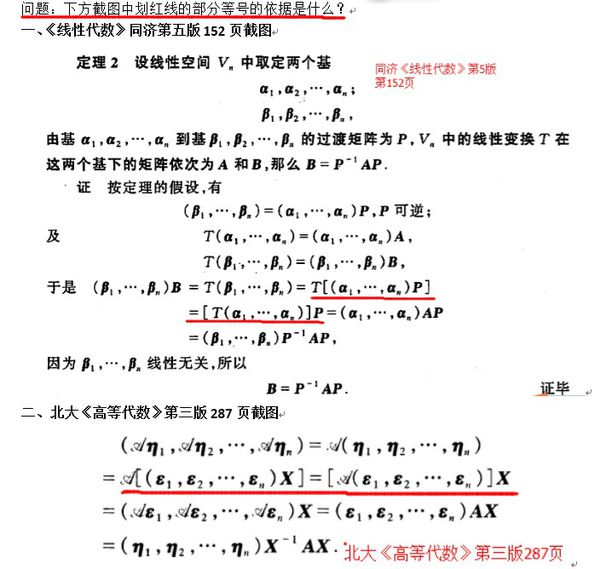
\includegraphics[width=0.90\textwidth]{similarproof.jpg}
\\
以及\url{https://www.bilibili.com/read/cv4496980/}。

所以
$$
T(\boldsymbol{W})=T(\boldsymbol{VP})= T(\boldsymbol{V [p_1,\cdots,p_n]})
=T(\boldsymbol{ [Vp_1,\cdots,Vp_n]})
$$
利用线性变换的性质——只作用于向量,不作用于线性组合的系数!这里$\boldsymbol{P}$的每个列向量都是
$\boldsymbol{V}$的列向量的组合系数,所以可以提出来!即
$$
=T(\boldsymbol{V})\boldsymbol{P}=\boldsymbol{VAP}\Rightarrow
\boldsymbol{WA}_{new}=\boldsymbol{VAP}=\boldsymbol{W}\boldsymbol{P}^{-1}\boldsymbol{AP}
\Rightarrow \underbrace{\boldsymbol{A}_{new}= \boldsymbol{P}^{-1}\boldsymbol{AP}}
$$

结论:如果是同一种线性变换,在不同基下对应的线性变换矩阵为$A,A_{new}$,则$A$与$A_{new}$\textbf{相似}。

注意:书上在此处的描述实际上对应$\boldsymbol{A}_{new}= \boldsymbol{P}^{-1}\boldsymbol{AP}
= (\boldsymbol{V}^{-1}\boldsymbol{W})^{-1}\boldsymbol{A}(\boldsymbol{V}^{-1}\boldsymbol{W})$,
因为书上指定输入基底$\boldsymbol{V=I}$,所以
$\boldsymbol{A}_{new}= \boldsymbol{W}^{-1}\boldsymbol{A}\boldsymbol{W}
\Rightarrow \boldsymbol{A}_{new}= \boldsymbol{B}^{-1}\boldsymbol{A}\boldsymbol{B}
$($\boldsymbol{B}$对应$\boldsymbol{W}$)。
\hspace*{\fill} \\

当输入空间$\boldsymbol{V}$和输出空间$\boldsymbol{W}$的维度不同时,对应线性变换$T$的矩阵$A$可能
不是对称阵,也不是方阵。但是可以通过选择基底来产生对应线性变换的对角阵(长方形对角阵)!

具体的做法:
通过选择奇异向量作为基底,即利用SVD——$U^{-1}AV=\Sigma_{m\times n}$,$\{\boldsymbol{v}_1,\cdots,\boldsymbol{v}_n\}$
作为输入基底;$\{\boldsymbol{u}_1,\cdots,\boldsymbol{u}_m\}$作为输出基底。

在原基底下的变换矩阵与选择奇异向量作为基底的变换矩阵相比:
$B_{\text {out }}^{-1} A B_{\text {in }}=U^{-1} A V=\Sigma$

总结:
最佳的输入-输出基底是变换矩阵A的特征向量或奇异向量,
$B^{-1} A B=\Lambda=$ eigenvalues $\quad B_{\text {out }}^{-1} A B_{\text {in }}=\Sigma=$ singular values
